\title{A Note on the Chorales}
\author{Hugh Zabriskie}
\documentclass[12pt]{article}
\usepackage{basecommon}
\usepackage{url}
\usepackage{tikz}
\urldef{\JSBChorales}\url{https://archive.ics.uci.edu/ml/datasets/Bach+Choral+Harmony}
\tikzset{
  treenode/.style = {shape=rectangle, rounded corners,
                     draw, align=center,
                     top color=white, bottom color=blue!20},
  root/.style     = {treenode, font=\Large, bottom color=red!30},
  env/.style      = {treenode},
  result/.style	={treenode, font=\Large, top color=blue!20, bottom color=blue!20}
}
\begin{document}
\maketitle


\section{The task and background}

The task is to compose 4-part chorales in the style of J.S. Bach given a 1-part melody. Bach composed over 300 harmonization of chorale melodies, and this corpus is used today for a variety of musicianship exercises, and in particular the composition of 4-voice counterpoint. The chorales are popular as a harmonization exercise for several reasons. Firstly, the sheer number of them is attractive to both musicians and computer scientists alike, and it is rare in music to find such a large collection of similarly structured compositions. Secondly, Bach's harmonizations exemplify many of the key properties of classical Western music, such as voice leading and cadential movement, and as such are thought to be excellent studies in Classical theory. And third, Bach broke as many as rules as he seemed to establish when composing these harmonizations, and these "irregularities" are what make the chorales interesting as compositions in their own right, rather than simply being academic exercises in counterpoint. \\

Recent work with the chorales has been based on a dataset named "JSB Chorales", which was generated by Allan \& Williams (2005), available at: \JSBChorales. Confusingly, there are two versions of the data. Version 1 is much smaller, only covering 60 chorales with a total of 5665 events, and provides information about the pitch classes, beat strength, bass note, and chord symbols for each event. Greff \& Schmidhuber (2015) used Version 1 to learn next-step prediction based on sequences of binary vectors, where each vector describes the pitch classes (i.e. 'C', 'C$\sharp$', 'D', etc.) present at some time step of a chorale. Radicioni \& Esposito (2010) also used Version 1 of the chorales to build BREVE, a system for chord labelling that mapped a collection of pitch classes to a chord symbol, and which they showed to be highly accurate.\\

The second version of JSB chorales consisted of 386 chorales stored as MIDI files and sampled once per beat, so that each chorale is represented as a sequence of beat-long time frames. Boulanger-Lewandowski et. al. (2012) used this version of the dataset, along with multiple other corpuses, to train several models on the task of music generation and to model temporal dependencies within polyphonic music (i.e. how distant musical events can be related). Each MIDI file was converted into a similar sequence of binary vectors, where each vector contained a list of MIDI numbers representing the notes that occurred at a specific time step. Liu (2014) also used the second version to "re-construct" chorales with an RNN by feeding chorales during training and then providing the beginning notes of each chorale in the test set as initial input to see if the rest of the composition could be re-composed - melody and harmony together.\\

Note that none of the recent papers described above work on the task of harmonization, but some work on related tasks such as chord identification and, more generally, music generation. Version 1 of the data does not identify the melody, only the pitch classes present and their corresponding chord symbol, making the task of harmonization impossible to learn on this data alone. Version 2, moreover, does not identify specific voices (i.e. it is unclear which voice belongs to the alto versus to the tenor) and the creators of the dataset only did a mediocre job at simplifying each chorales into a series of representative chords at each step. The data used in this paper improves upon this version by more carefully "quantizing" the chorales into sequences of beat-long time frames while also identifying each note with one of the 4 voices. The most well-known attempts at chorale harmonization in the last decade did not use neural networks in their models. Allan \& Williams (2005) used Hidden Markov Models with reasonable success and Buys \& Merwe (2012) used weighted finite-state transducers (WFST) and had results "competitive" with Allan \& Williams.  \\ 

In short, the original task of harmonizing chorales, has not been approached as effectively or thoughtfully, in the opinion of the author, since the HARMONET system was published by Hild, Feulner, and Menzel in 1992. HARMONET completes the task of harmonization using 3 neural nets where the output of one is fed as input to the next. The first network selects a "harmonic skeleton" that outlines the harmonies for the entire chorale, the second net selects the alto and tenor voices, and the final net adds rhythmic ornamentation (i.e. passing tones) to better model the rhythmic patterns in Bach's original harmonizations. In all recent papers, rhythmic complexity has been entirely factored out to focus on other aspects of the music. While HARMONET was not evaluated qualitatively, the chorales it produced were judged to be "on the level of an improvising organist" - a rather glowing review. Moreover, it was only trained on 40 chorales (split evenly between major and minor keys) rather than the entire collection of chorales. Therefore, in many ways HARMONET provides a strong model for approaching the task of harmonization while also leaving room for improvement. since neural networks and the field of machine learning generally have developed significantly since this model was published.

\subsection{The task computationally}

Mathematically, let's define the task more concretely. The algorithm should take as input the chorale, represented a sequence of notes, and it should output a corresponding sequence of 3-voice chords that represent the alto, tenor, and bass voices. Following the approach of HARMONET, the task is divided into 3 steps:
\begin{enumerate}
\item Creation of a harmonic skeleton in the form of Roman numeral analysis. This also implies a bass line.
\item The selection of the alto voice.
\item The selection of the tenor voice.
\end{enumerate}
We assume that we are given a sequence of symbols from a vocabulary $V$. That sequence represents an entire chorale.
$$x_1, x_2, x_3, \ldots \quad x_i \in V$$
Each symbol $x_i$ describes a set of features about the melody at time $i$. Those features include, but need not be limited to:
\begin{itemize}
\item The pitch of the melody at time $i$. Optionally, pitches that comes directly before or after it as well ($i-1$, $i+1$).
\item The beat strength, to add metrical context (i.e. is it on a downbeat?).
\item Whether a cadence occurs at time $i$, represented by a fermata.
\item Chorale-specific information, such as the key signature and time signature.
\end{itemize}

\noin Let's say we have $m$ data points with $n$ features, and $Y$ output classes.
\begin{itemize}
\item $\boldX \in V^{m \times n}$ is our input data
\item $\boldY \in Y^m$ is our output data
\end{itemize}

\subsection{Recurrent model}

Another potential source of information in a recurrent model is the harmony chosen in the previous computation for time $i-1$. Many papers have suggested the importance of knowing previous chosen harmonies in predicting subsequent harmonies, which is in line with the musical conception of harmony as a \textit{progression}. Often in Western music, and always within the chorales, a chord or harmony is viewed within the context of its surrounding harmonies, a component in a progression. We treat the importance of the preceding harmonies as a hypothesis. And this hypothesis is tested by an "Oracle experiment" that examines whether a baseline model improves when trained with the knowledge of the harmony that directly precedes it.    

\section{Baseline model}

To determine a baseline accuracy for the harmonization task, 3 classifiers were trained: naive Bayes, multi-class logistic regression, and a 3-layer non-recurrent network.

\subsection{Subtask: Generating a harmonic skeleton} 

The harmonic skeleton is composed of two complimentary sets of decisions: a choice of harmony, represented as a Roman numeral, and a choice of inversion. Information about the chosen harmony was provided in learning the inversion. This two-part decision process resembles a musician's approach to 4-part counterpart, who would decide upon a harmonic progression and then smooth the bass line with the use of inversion. \\

In order to generate the data, Roman numeral analysis was performed across the entire corpus of chorales using the \texttt{roman} Python module of music21, combined with manual correction and minimal simplification of the harmonic output classes.

\begin{center}
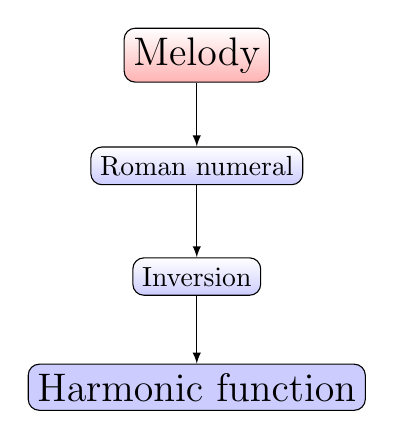
\begin{tikzpicture}
  [
    grow                    = down,
    sibling distance        = 6em,
    level distance          = 4em,
    edge from parent/.style = {draw, -latex}
  ]
  \node [root] {Melody}
    child { node [env] {Roman numeral} 
    	child { node [env] {Inversion} 
		child { node [result] {Harmonic function} }}};
\end{tikzpicture}
\end{center}

\subsection{Numeral subtask}

For Roman numeral selection, each melody note was assigned one of 54 possible Roman numerals. Using \texttt{scikit-learn}, a naive Bayes classifier and a multi-class logistic regression classifier were trained on the data. \texttt{eval\_num.lua} includes a Torch implementation of both the logistic classifier and a non-recurrent network with one hidden layer. Hyperparameters for the network were optimized to a learning rate of $0.01$, and both a hidden layer and embedding size of $250$.

\begin{center}
	\begin{tabular}{ c | c | c }
		\textbf{Classifier} & \textbf{Accuracy - Training Set} & \textbf{Accuracy - Test Set} \\ \hline
		Multi-Class Logistic & 36.23\% & 31.50\% \\ \hline
		Naive Bayes & 31.78\% & 28.19\% \\ \hline
		Neural Network & 70.77\% & 46.46\%
	\end{tabular}
\end{center}	

The average NLL for training was 0.787 and 2.001 was testing. Note that predicting the most frequent class would give an accuracy of 18\% on the training set and 21\%  on the test set, so the model is clearly learning. An NLL of 0.787 means that the model gives approximately 45\% of the weight to the correct answer during training.

An Oracle experiment was then performed to see if knowing the correct previous harmony would improve accuracy. The hypothesis is that the previous decision is not independent of the current decision because in the chorales each harmony is one element of a harmonic \textit{progression}, or a sequence of inter-related harmonies. The 6\% increase in accuracy hypothesis proved to be true, suggesting that a recurrent model could significantly improve classification accuracy because of its ability to model sequences of data.

\begin{center}
	\begin{tabular}{ c | c | c | c }
		\textbf{Classifier} & \textbf{Training} & \textbf{Test} & \textbf{Accuracy $\Delta$}\\ \hline
		Multi-Class Logistic & 45.19\% & 40.71\% & 9.21\% \\ \hline
		Naive Bayes & 41.22\% & 36.95\% & 8.76\% \\ \hline
		Neural Network ("oracle") & 80.61\% & 52.52\% & 6.06\%
	\end{tabular}
\end{center}


\subsection{Inversion subtask}

For inversion selection, each melody note and the correct corresponding Roman numeral were assigned one of 13 possible inversions. In this task, predicting the most frequent class (root position) would already give you 57\% accuracy on both the training and test sets. The same 3 classifiers were used. For the network, the validation set was used to tune the parameters to an embedding size and hidden unit size of 200 and a learning rate of 0.001.

\begin{center}
	\begin{tabular}{ c | c | c }
		\textbf{Classifier} & \textbf{Training} & \textbf{Test} \\ \hline
		Multi-Class Logistic & 63.23\% & 64.68\% \\ \hline
		Naive Bayes & 60.35\% & 60.92\% \\ \hline
		Neural Network & 74.56\% & 66.01\%
	\end{tabular}
\end{center}

\subsection{Alto and Tenor subtasks}

The same model was applied to classifying the alto and tenor notes, separately. These models yielded a test accuracy of 35.06\% on for the alto voice and 29.22\% for the tenor voice. 

\subsection{Classifier Sequence}

4 classifiers were trained separately, once for each subtask (numeral, inversion, alto, tenor). During evaluation the output of each classifier was passed as part of the input to the next classifier, to represent the full sequence of harmonic decisions.

\begin{center}
	\begin{tabular}{ c | c | c }
		\textbf{Task} & \textbf{Average NLL} & \textbf{Accuracy} \\ \hline
		Roman numeral & 2.316 & 45.04\% \\ \hline
		Inversion & 2.558 & 48.50\% \\ \hline
		Alto & 2.595 & 34.76\% \\ \hline
		Tenor & 5.074 & 23.56\% \\ \hline
		Numeral + inversion & -- & 26.11\% \\ \hline
		All 4 & -- & 3.10\%
	\end{tabular}
\end{center}


\end{document}